\documentclass[a4paper,11pt,oneside]{article}
\usepackage{gensymb}
\usepackage{geometry}
 \geometry{
 a4paper,
 total={155mm,247mm},
 left=30mm,
 top=25mm,
 }

\usepackage[utf8]{inputenc}
\usepackage{graphicx}

\title{\textbf{Volcanism on Jupiter's moon Io}}
\author{\textbf{Kiran Tikare} \\ Lulea University of Technology, Sweden \\ {kirtik-3@student.ltu.se}}

\date{October 2018}

\begin{document}

\maketitle 

\newpage
\tableofcontents
\newpage
\thispagestyle{empty}
 
\listoffigures
 
\listoftables
\newpage

\section{Introduction}
Ever since Galileo Galilei pointed his telescope towards Jupiter and made observations of Jupiter and discovered its moons - called galilean moons - a sort of mini solar system, it has improved our knowledge of the solar system tremendously. Since Galileo's time until now many ground based, space based measurements have been carried out in studying Jupiter and its moons. Gas giant Jupiter is one of the biggest planet in our Solar System and has at least 67 moons. Among them Io is the innermost moon and is most geologically active body in the Solar System and more than 400 volcanoes have been detected so far on Io. Io is in 1:2:4 orbital resonance with other 2 moons Europa and Ganymede. Io lies within the Jupiter's magnetosphere and undergoes tidal effects due to Jupiter and its moons. These tidal forces drive volcanism of Io. Volcanism on Io was discovered by Linda Morabito from the image captured by Voyager 1 spacecraft during flyby.

\section{Historical Background}
In the year 1610 Galileo Galilie while observing the planet Jupiter noticed tiny stars and he also noticed they were going around Jupiter. He published his discoveries in his work "Sidereus Nunceus" written in March 1610 and named these little stars as "Cosmica Sidera" (Cosimo's Stars), after the King Cosimo Medici. Later On insistance of Cosimo Medici he changed the names to "Medicina Sidera" ("Medician Stars"). Simon Marius in his work “Mundus Jovialis" published in 1614 claimed to have discovered these moons independently. On the suggestion of Johannes Kepler Marius named these moons after lovers of Zeus as Io, Europa, Ganyemede, Calisto. AS the Galileo's work was published before Marius, Galileo is credited with the discovery of Jupiter's moons, now known as "Galilean Moons" and scientific community has adopted names given by Marius.

Since the days of Galileo and Marius Jupiter and its moons have helped astronomers determine the speed of light, determination of longitude to name a few instances.



\section{Orbital and Physical Characteristics}
\subsection{Orbital Characteristics}
Io is the inner most satellite of Jupiter and is located at a distance of 421,700 km from the centre of Jupiter. Io lies almost at the same distance from Jupiter as our own Moon from Earth. Io is not only under the gravitational influence of Jupiter but also the other neighbouring moons Europa, Ganymede, Calisto.  For every 4 orbits that Io makes around Jupiter, Europa goes around Jupiter twice and, for every 2 orbits of Io, Ganymede goes around Jupiter once. Periodically they line up together and this puts Io under the pressure of tremendous gravitational force on regular basis.  This produces eccentricity in the orbit of Io. Io is tidally locked to Jupiter so one face is always pointing towards Jupiter. This is used to define hemispheres of Io, the side facing the Jupiter is SubJovian Hemishphere and the other side is Anti-Jovian Hemisphere. The figure \ref{fig:orbres} shows the orbits of Io, Europa, Ganymede for a period of 8 days. 

 

\begin{figure}[ht]
\centering
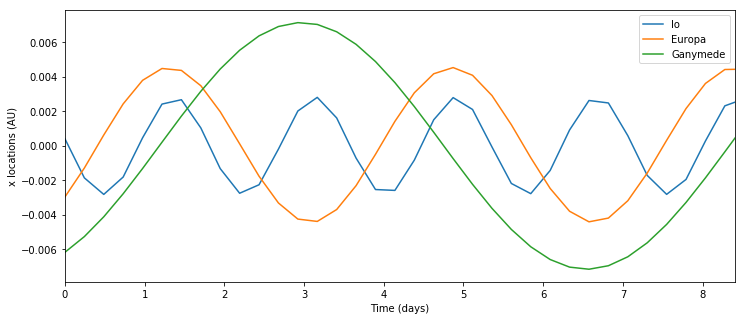
\includegraphics[width=0.9\textwidth]{figures/orb-res.png}
\caption{Orbits of Io, Europa, Ganymede are in 1:2:4 Laplace Resonance.}
\label{fig:orbres}
\end{figure}

\begin{table}[ht]
\centering
\begin{tabular}{ll}
\textbf{Property} & \textbf{Values}  \\
Periapsis & 420,000 km (0.002807 AU) \\
Apoapsis & 423,400 km (0.002830 AU) \\
Mean Orbit Radius & 421,700 km (0.002819 AU) \\
Eccentricity & 0.0041 \\
Orbital Period & 1.77 days \\
Inclination & 0.05 \degree (to Jupiter's equator) \\
Avg. Orbital Speed & 17.334 km/s
\end{tabular}
\caption{Orbital Properties of Io}
\label{table:1}
\end{table}



\subsection{Atmospheric Composition}
\subsection{Surface Features}
The figure \ref{fig:iofulldiscvoyager1} shows full disc of Io as seen by Voyager 1 spacecraft. One can notice that the surface is young as there are no craters. The lava from the volcano's flow over the surface and produce new surface. 
\begin{figure}[ht]
\centering
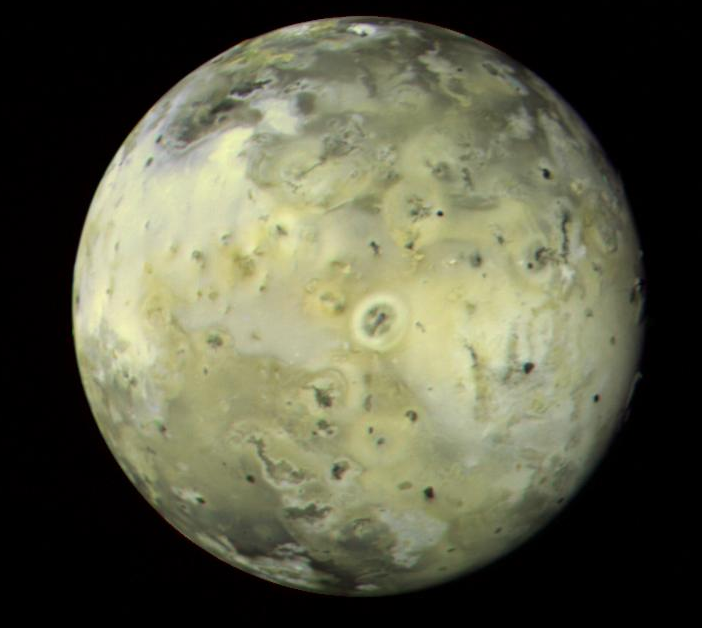
\includegraphics[width=0.6\textwidth]{figures/fulldiscvoy1.png}
\caption{Full disc of Io as seen by Voyager 1 spacecraft.\cite{iofulldiscvoyager1} Image Credit:NASA/JPL}
\label{fig:iofulldiscvoyager1}
\end{figure}
The peculiar color is the result of sulphur deposits on the surface.

\begin{table}[ht]
\centering
\begin{tabular}{ll}
\textbf{Property} & \textbf{Values}  \\
Mean radius & 1,821 km (0.286 Earths) \\
Surface area & 41,910,000 km\textsuperscript{2} (0.082 Earths) \\
Volume & 2.53x10\textsuperscript{10} km\textsuperscript{3} (0.023 Earths) \\
Mass & (8.9)x10\textsuperscript{22} kg (0.015 Earths) \\
Mean Density & 3.5 g/cm\textsuperscript{3} \\
Surface Gravity & 1.796 m/s\textsuperscript{2} \\
Escape Velocity & 2.558 km/s \\
Rotation Period & Syncrhonous\\
Albedo & 0.63\\
Surface Temperature & 90K to 130K \\
Appearant Magnitude & 5.02 (Opposition)
\end{tabular}
\caption{Physical Properties of Io}
\label{table:2}
\end{table}

\subsection{Internal Structure}
The figure\ref{fig:iointernal} shows artist impression of the internal structure.
\begin{figure}[ht]
\centering
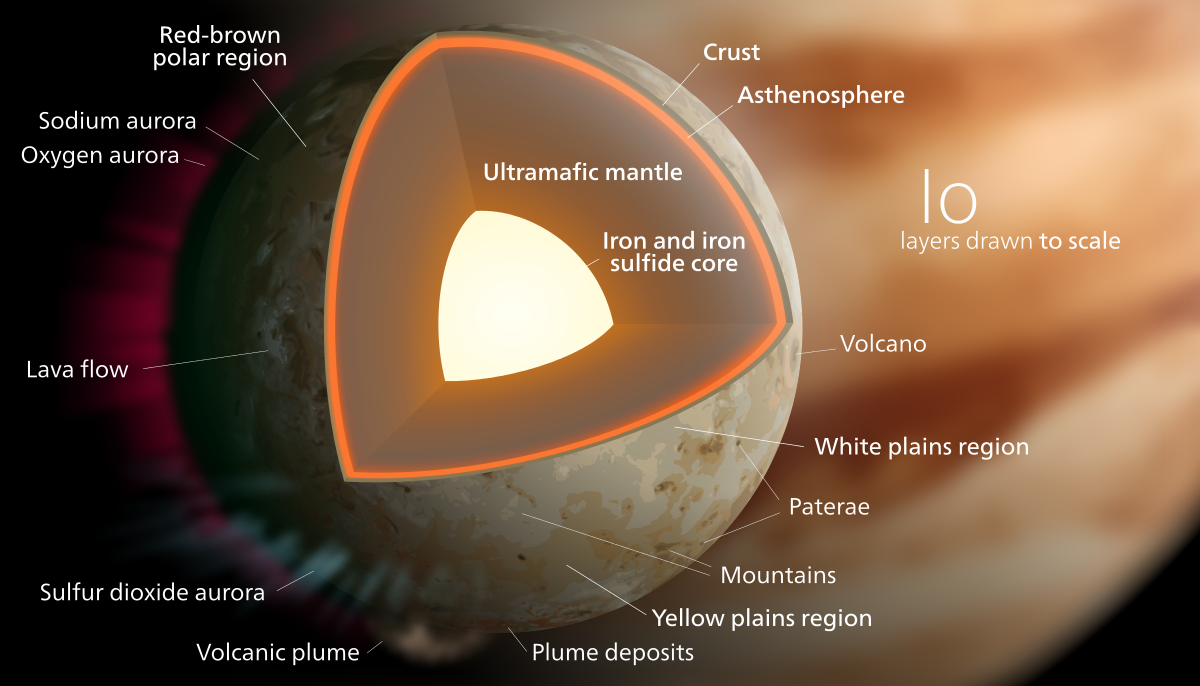
\includegraphics[width=0.8\textwidth]{figures/io-internal.png}
\caption{Artists impression of Io's interior. Image Credit : Wikipedia}
\label{fig:iointernal}
\end{figure}
\newline
\section{Observations}
\subsection{Ground Based Observation}
In most of the history of Astronomy, discoveries were made based on the ground based observations. Since the discovery of Io by Galileo and Marius up until 19\textsuperscript{th} century, Jupiter and its moons have been target of many ground based observations. Until the 19\textsuperscript{th} century Io remained a distant 5\textsuperscript{th} magnitude mysterious moon without much insights. With the rise of Radio Astronomy, many turned to study Jupiter and its moons.

\subsection{Space Based Observation}
Jupiter and its moon have been target of few of the Space Missions so far. Table \ref{table:3} lists some of the space missions which made few studies of the Jupiter and its moons. Some of the Space Missions such as Pioneer (10 and 11), Voyager (1 and 2), Ulysses, Cassini-Hyugens, New Horizons visited Jupiter during their mission life time and some Space Missions like Galileo, JUNO were specifically sent to study Jupiter and its moons. These visitations have tremendously improved our knowledge and understanding of the mysterious moons of Jupiter.

\begin{table}[ht]
\begin{tabular}{lll}
 \textbf{Mission} & \textbf{Operating Period}  & \textbf{Io Flyby's}  \\
 Pioneer 10 & 2 March 1972 - 27 April 2002 &  \\
 Pioneer 11 & 5 April 1973 - November 1995 &  \\
 Voyager 1 & 5 September, 1977 - Present &  \\
 Voyager 2 & 20 August 1977 - Present &  \\
 Galileo & 18 October 1989 - 21 September 2003 &  \\
 Ulysses & 6 October 1990 - 30 June 2009&  \\
 Cassini–Huygens & 15 October 1997 - 15 September 2017 & \\
 New Horizons & 19 January 2006 - Present &  \\
 JUNO & 5 August 2011 - Present & 
\end{tabular}
\caption{Space Missions that made Observations of Jupiter and Its Moons}
\label{table:3}
\end{table}

\subsubsection{Discovery of Volcanism}
The figure \ref{fig:iovolc} shows an image captured by Voyager Spacecraft. This image was used by Linda A Morabito who was working at the NASA's Jet Propulsion Laboratory as a Voyager Navigation Engineer, to discover the volcanic plume.\cite{morabito}. 

\begin{figure}[ht]
\centering
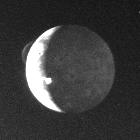
\includegraphics[width=0.6\textwidth]{figures/PIA00379.jpg}
\caption{Volcanic eruptions on Io, image used by Linda A. Morabito JPL engineer at that time to discover extraterrestrial volcanic eruption. Image Credit : NASA/JPL}
\label{fig:iovolc}
\end{figure}

\begin{figure}[ht]
\centering
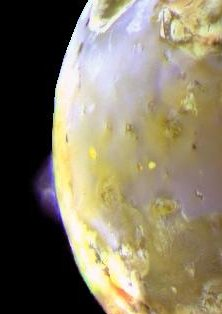
\includegraphics[width=0.6\textwidth,height=0.6\textwidth,keepaspectratio]{{figures/plume.jpg}}
\caption{Volcanic plume as seen by Galileo Spacecraft. Image Credit : NASA/JPL}
\label{fig:iovolcplume}
\end{figure}


\subsubsection{Future Missions}

\section{Volcanism on Io}
\subsection{Jupiter and Io interactions}
Io not only undergoes gravitational interaction with Jupiter but also significantly contributes gas and dust to its Magnetosphere. The gas and dust particles from volcanic plumes from Io's atmosphere are picked up by Jupiter's magnetosphere and are transported back to Jupiter where they rotate under the influence of Jupiter's gravitational field producing Palsma Torus around Jupiter.

Studies done on the data collected by Ulysses's fly by and then Galileo mission, proved that Io as a major contributor to Jovian Dust Stream.\cite{graps} This dust gets picked up by Jupiter's magnetic field and a Plasma Torus is formed around Jupiter.

\subsubsection{Io Plasma Torus (IPT)}
 It is doughnut shaped ring of plasma and is rotating with the Jupiter at the orbit of Io and is largely composed of ionised oxygen and sulfur atoms which were released by Io's volcano's. Ulysses made IPT measurements during its flyby and was able to confirm the scientific conclusions of Voyager Mission data.

\newpage

\section{Bibliography}
\begin{thebibliography}{9}
\bibitem{morabito}
Linda A. Morabito. 
\textit{Discovery of Volcanic Activity on Io - A Historical Review}. 
arXiv:1211.2554v1, 2012.

\bibitem{morabito1}
Linda A. Morabito et al., 
\textit{Discovery of Currently Active Extraterrestrial Volcanism}. 
Science, 1979, Vol 204, Issue 4396, pp. 972.

\bibitem{peale}
Peale,S.J., et al., 
\textit{Melting of Io by Tidal Dissipation}. 
Science, 1979, Vol 203, pp 892-894.

\bibitem{volcanodiscpic} 
Voyager's Io image used for Discovering Volcanic Plume,
\\\texttt{https://photojournal.jpl.nasa.gov/catalog/PIA00379}, Accessed on 14 October 2018

\bibitem{iofulldiscvoyager1} 
Io's full disc taken by Voyager 1,
\\\texttt{https://photojournal.jpl.nasa.gov/jpeg/PIA00023.jpg}, Accessed on 14 October 2018

\bibitem{graps}
A. L. Graps., et al., 
\textit{Io as a source of the jovian dust streams}. 
Nature volume 405, pages 48–50 (04 May 2000).

\bibitem{mcewen}
McEwen,A. S., et al., 
\textit{Active volcanism on Io as seen by Galileo}. 
SSI. Icarus 135, 181–219 ( 1998).

\end{thebibliography}


\end{document}
